\documentclass{article}

\usepackage[skip=20pt, indent=0pt]{parskip}
\usepackage{xcolor, graphicx, afterpage}
\usepackage{amsmath, eqparbox, bm, mathtools, tensor, amsfonts}
\usepackage{algpseudocode, algorithm}
\usepackage{multirow}
\usepackage{hyperref}

\author{écrit par \\ \\ \textbf{TAMDRARI Yacine} \\ \\ Révisé par \\ RZESZUTEK Christian 
et FITZGERALD Avon}
\title{\Huge{\textbf{\textcolor{blue}{Le code de Hadamard}}}}

\begin{document}

\maketitle
\begin{figure}
\begin{center}

\includegraphics[width=0.4\textwidth]{logo.png}
\label{logo paris cité}
\end{center}
\end{figure}
\newpage
\titlepage

\tableofcontents
\newpage

\section{Introduction}

\subsection{Definition}

Le code de Hadamard nommé d'aprés le mathématicien Français Jacques
Hada\-mard est un code correcteur d'erreur linéaire (le plus connu mais il 
existe des codes de Hadamard non linéaire) utilisé dans plusieurs 
domaines tels que le traitement de signal, le cryptage et la 
télécommunication; il a été utilisé le 14 novembre 1971 pendant la mission
du visseau spataial Mariner 9 pour corriger les erreurs de transmission des
images depuis l'orbite de Mars.

\begin{figure}[h]
\begin{center}
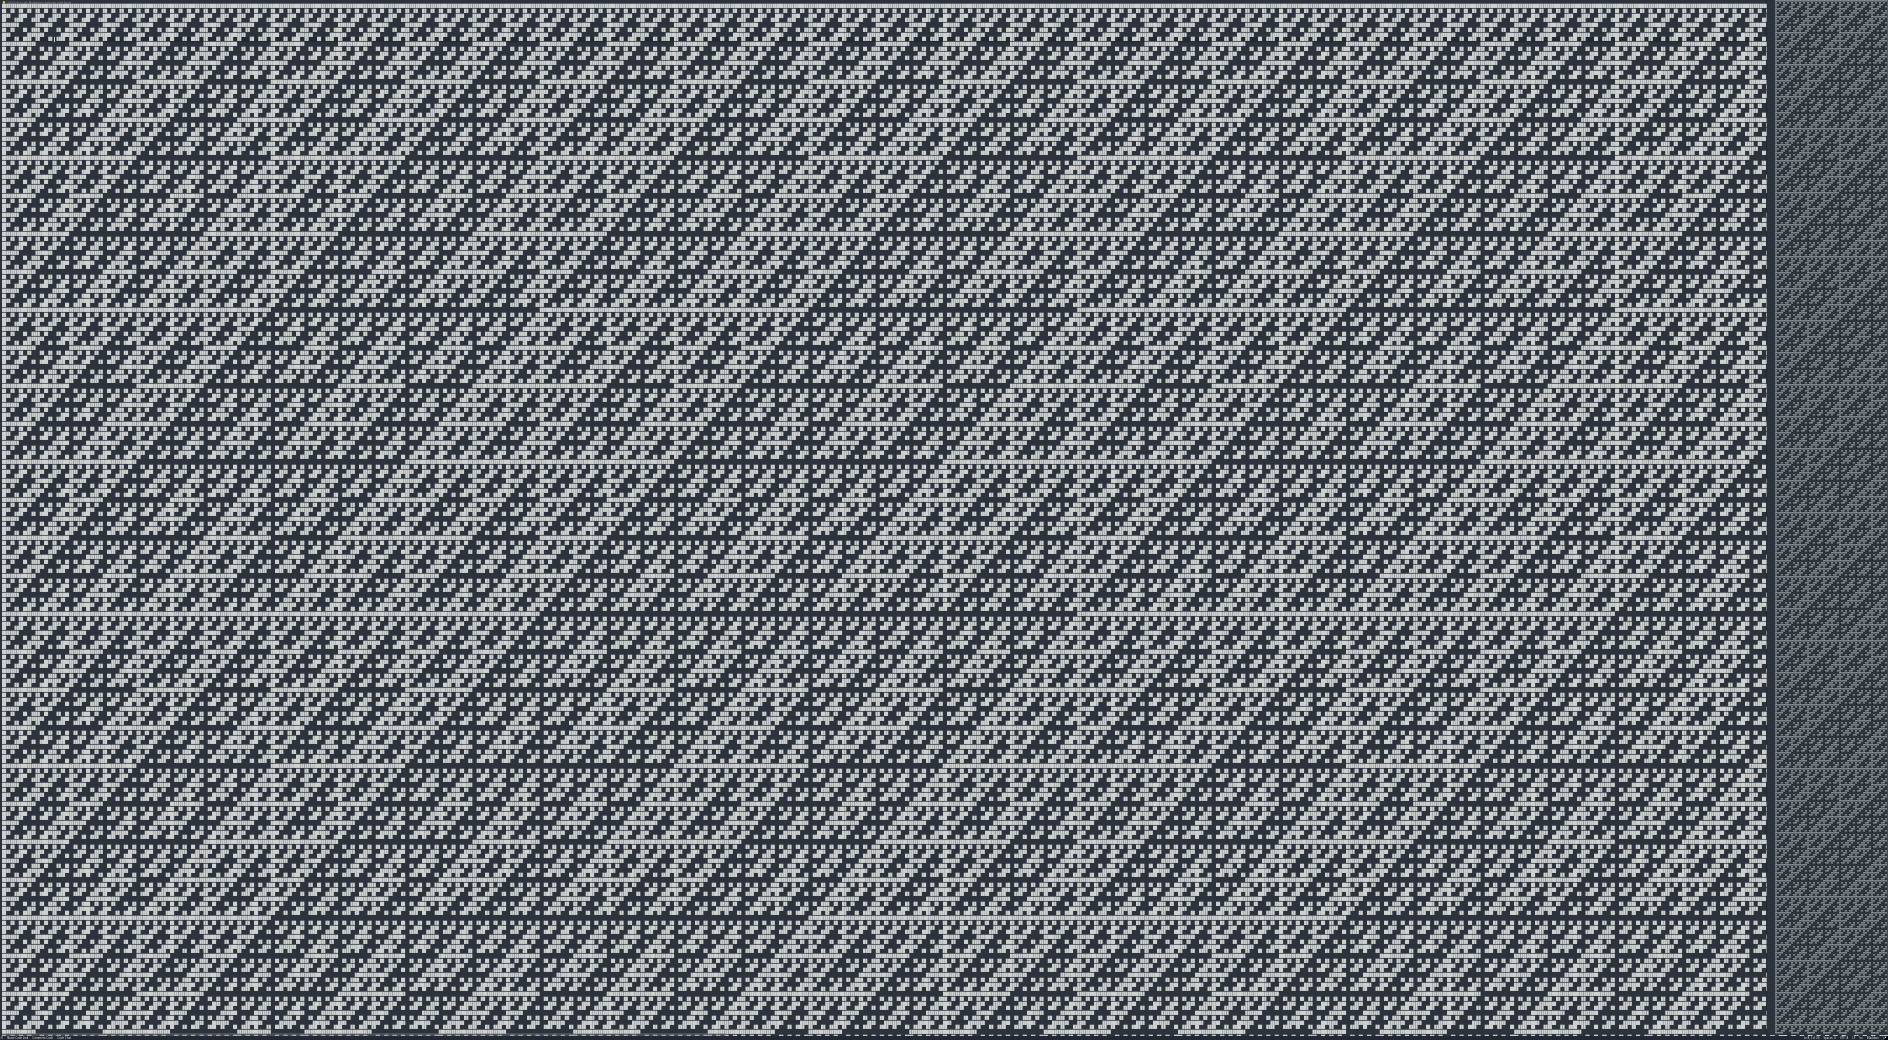
\includegraphics[width=1\textwidth]{hadamard.png}
  \caption{Une partie d'une matrice Hadamard d'ordre 10 (Cette matrice est construite avec le programme fourni sylvester.ml)}
  \label{hadamard d'ordre 10}
\end{center}
\end{figure}

\subsection{Le code de Hadamard en théorie}

Le code de Hadamard est un code sur un alphabet de taille $2^k$ ou k est un
entier positif, chaque mot du code a une longueur de k bits donc pour coder
une information avec k bits le code ajoute $2^k$-k bits pour former un mot
de code sur $2^k$ bits, ceci implique que pour transférer k bits 
d'informations avec ce code le taux de transfert sera $\frac{k}{2^k}$ qui
est extrêmement faible donc rends le temps de transmission des informations
lent, mais le code est couramment utilisé à cause de sa capacité à détecter
toutes les erreurs simples car la distance de Hamming\footnote{le nombre 
de bits différents entre deux mots de code binaires qui peut etre trouvé en
sommant les résultats des XOR $\oplus$ bit à bit des deux mots de code} entre deux séquences de 
code est $\frac{n}{2}$ = $\frac{2^k}{2}$ = $2^{k-1}$ cela 
signifie que le code serait capable de détecter jusqu'à $2^{k-1}$ erreurs 
simples, un code correcteur à une distance de Hamming d est capable de 
corriger $\frac{d-1}{2}$ erreurs ce qui donne $\frac{2^{k-1}-1}{2}$ pour le
code de Hadamard (pour avoir une correction il faut que $k>2$ donc ce code 
serait fiable sur des canaux trés bruyants sur lequels le risque de 
corruption d'une information est trés grand; dans la notation standard de 
la théorie du codage pour les codes en bloc on note ceci avec 
$[2^k, k, 2^{k-1}]_2$.

\subsection{Un peu d'histoire}

Le code de Hadamard est le nom le plus couramment utilisé pour ce code dans
la littérature bien que Jacques Hadamard n'a pas inventé le code de 
lui-meme mais il a initié les bases de ce code en déffinissant les matrices
d'Hadamard vers 1893, bien avant que le premier code correcteur d'erreurs
(le code de Hamming vers 1940) ne soit développé.

Il existe plusieurs construction des matrices d'Hadamard mais la plus 
utilisée est celle définie par James Joseph Sylvester en 1867 qui est en 
fait antérieure aux travaux d'Hadamard sur ses matrices, des codes 
d'Hadamard non linéaires ont été construit par R. C. Bose et S. S. 
Shrikhande en 1959.

\subsection{Application dans la vie réelle}

Un code Hadamard a été utilisé lors de la mission Mariner 9 de 1971 pour
corriger les erreurs de transmission d'images; les mots de données 
utilisés au cours de cette mission étaient de 6 bits, ce qui représentait 
64 valeurs en niveaux de gris.En raison des limitations de la qualité de 
l'alignement de l'émetteur, la longueur maximale des données utiles était 
environ 30 bits.Au lieu d'utiliser un code de répition, un code Hadamard
a été utilisé.Des erreurs allant jusqu'à 7 bits par mot pourraient etre 
corrigées à l'aide de ce code; par rapport à un code à 5 répétitions, les
propriétés de correction d'erreurs de ce code Hadamard sont bien meilleures
mais son taux est comparable.L’efficacité de l’algorithme de décodage a été
un facteur important dans la décision d’utiliser ce code.Le circuit 
utilisé s'appelait la \textbf{machine verte}.Il utilisait la transformée de
Fourier rapide qui peut augmenter la vitesse de décodage d'un facteur 3.
Depuis les années 1990, l'utilisation de ce code par les programmes 
spatiaux a plus ou moins cessé, et le Deep Space Network ne prend pas en 
charge ce système de correction d'erreurs pour ses antennes paraboliques.
mesurent plus de 26 m.

\section{Les matrices d'Hadamard}

\subsection{Introduction}
Une matrice Hadamard est une matrice carré de taille $n*n$ avec des entrées
dans l'ensemble \{-1; 1\} qui a plein de propriétés que nous détailleront 
dans la suite de cet article.

Les matrices d'Hadamard exercent sur nous une fascination depuis un siécle
et demi, transparentement faciles à décrire, omniprésentes et utilitaires;
dans la vie quotidienne ces matrices sont largement utilisées, la 
transformée de Walsh-Hadamard est couramment utilisée comme transformulaire
, elles ont été utilisée dans les premières transmissions par satellite 
pour former des codes correcteurs, les téléphones portables CDMA utilisent 
ces matrices pour moduler la transmission, aussi utilisées dans le domaine
de la communication optique et la dissimulation d'informations...

La conjuncture de Hadamard annonce que pour tout nombre naturel n, il 
existe une matrice d'Hadamard d'ordre $4*n$, reste l'un des grands 
problémes non résolus de mathématiques; detaillons quelques propriétés de 
ces matrices et les méthodes de leurs constructions.

\textbf{example:} Les matrices d'Hadamard d'ordre 2 et 4:\\

\begin{equation*}
\mathcal{H}_2 = \begin{bmatrix}
	1 & 1\\
	1 & -1
\end{bmatrix}
\quad
\mathcal{H}_4 = \begin{bmatrix}
	1 & 1 & 1 & 1\\
	1 & -1 & 1 & -1\\
	1 & 1 & -1 & -1\\
	1 & -1 & -1 & 1
\end{bmatrix}
\end{equation*}

\subsection{Propriétés}

\subsubsection{Orthogonalité}

Chaque ligne et chaque colonne d'une matrice de Hadamard sont orthogonales
entre elles c'est à dire le resultat du produit scalaire de chaque deux 
lignes ou de chaque deux colonnes est nul.

Par exemple l'orthogonalité entre la premiére ligne de $\mathcal{H}_4$ et 
la troisième ligne de la meme matrice est:
\begin{equation*}
	\begin{pmatrix}
		1\\
		1\\
		1\\ 
		1
	\end {pmatrix}
	.
	\begin{pmatrix}
		1 & 1 & -1 & -1\\ 
	\end{pmatrix}
	= 1*1+1*1+1*(-1)+1*(-1) = 0. 
\end{equation*}

\subsubsection{La transposée d'une matrice Hadamard}

Toutes les matrices d'Hadamard ont la propriété suivante:
\begin{equation}\label{eq:transposée}
	\mathcal{H}_n . \mathcal{H}_{n}^{\mathcal{T}} =
	\mathcal{H}_{n}^{\mathcal{T}}. \mathcal{H}_n = n.\mathcal{I}
\end{equation}
ou $\mathcal{I}$ est la matrice identité de taille n et 
$\mathcal{H}_{n}^{\mathcal{T}}$ la transposée de $\mathcal{H}_n$.

Par exemple:
\begin{equation*}
	\mathcal{H}_2 . \mathcal{H}_{2}^{\mathcal{T}} =
	\begin{bmatrix}
		1 & 1\\
		1 & -1
	\end{bmatrix}
	.
	\begin{bmatrix}
		1 & 1\\
		1 & -1
	\end{bmatrix}
	=
	\begin{bmatrix}
		2 & 0\\
		0 & 2
	\end{bmatrix}
	= 2 . \mathcal{I}
\end{equation*}

\subsubsection{L'inverse d'une matrice Hadamard}

Il est facile de trouver l'inverse d'une matrice Hadamard, en effet d'aprés
l'équation (\ref{eq:transposée}):
\begin{equation*}
	\mathcal{H}_n . \mathcal{H}_{n}^{\mathcal{T}} = n * \mathcal{I}
	\quad
	donc 
	\quad
	\mathcal{H}_n . \frac{1}{n}*\mathcal{H}_{n}^{\mathcal{T}} = \mathcal{I}
	\quad
	\text{d'ou le résultat:} 
\end{equation*}
\begin{equation}\label{eq:inverse}
	\mathcal{H}_{n}^{-1} =  \frac{1}{n}*\mathcal{H}_{n}^{\mathcal{T}}
\end{equation}

\subsubsection{Déterminant d'une matrice Hadamard}

Si $\mathcal{M}$ est une matrice d'ordre $n$ dont les coefficients sont 1 
et -1, alors d'aprés la majoration de Hadamard:
\begin{equation}
	\det(\mathcal{M}) \leq n^{\frac{n}{2}}
\end{equation}
$\mathcal{M}$ est une matrice d'Hadamard si et seulement si elle atteint 
l'égalité d'Hadamard, c'est à dire: 
$|\det(\mathcal{M})| = n^{\frac{n}{2}}$

\subsubsection{Trace d'une matrice Hadamard}

Si $\mathcal{H}_n$ est une matrice d'Hadamard d'ordre $n$ alors sa trace 
est nulle:
\begin{equation}\label{eq:trace}
	\mathrm{tr}(H_n) = 0
\end{equation}

\subsubsection{Produit de Hadamard}

Le produit de Hadamard est une opération binaire qui pour deux matrices de
meme dimensions, associe une autre matrice de meme dimension, formellement:
\begin{equation*}
	\begin{bmatrix}
		a_{1,1} & a_{1,2} & \cdots & a_{1,m}\\
		a_{2,1} & a_{2,2} & \cdots & a_{2,m}\\
		\vdots & \vdots & \ddots & \vdots\\
		a_{n,1} & a_{n,2} & \cdots & a_{n,m}
	\end{bmatrix}
	o
	\begin{bmatrix}
		b_{1,1} & b_{1,2} & \cdots & b_{1,m}\\
		b_{2,1} & b_{2,2} & \cdots & b_{2,m}\\
		\vdots & \vdots & \ddots & \vdots\\
		b_{n,1} & b_{n,2} & \cdots & b_{n,m}
	\end{bmatrix}
	=
	\begin{bmatrix}
		a_{1,1}*b_{1,1} & a_{1,2}*b_{1,2} & \cdots & a_{1,m}*b_{1,m}\\
		a_{2,1}*b_{2,1} & a_{2,2}*b_{2,2} & \cdots & a_{2,m}*b_{2,m}\\
		\vdots & \vdots & \ddots & \vdots\\
		a_{n,1}*b_{n,1} & a_{n,2}*b_{n,2} & \cdots & a_{n,m}*b_{n,m}
	\end{bmatrix}
\end{equation*}

Le produit matriciel de Hadamard est associatif et distributif, et 
contrairement au produit matriciel classique, commutatif. 

Le produit de deux matrices Hadamard est une matrice Hadamard.

\subsection{Construction}

\subsubsection{Produit de Kronecker}

Le produit de Kronecker $\otimes$ de deux matrices $\mathcal{A}$ et 
$\mathcal{B}$ de taille respectivement $m*n$ et $p*q$, avec 
$m, n, p, q \in \mathbb{R}$ résulte une matrice de taille $mp*nq$ définie
par:

\begin{equation*}
	\mathcal{C} = \mathcal{A} \otimes \mathcal{B}
	\quad
	\text{tel que;}
	\quad
	\mathcal{C} =
	\begin{pmatrix}
		a_{1,1}*B & a_{1,2}*B & \cdots & a_{1,n}*B\\
		a_{2,1}*B & a_{2,2}*B & \cdots & a_{2,n}*B\\
		\vdots & \vdots & \ddots & \vdots\\
		a_{m,1}*B & a_{m,2}*B & \cdots & a_{m,n}*B
	\end{pmatrix}
\end{equation*}

Exemple:

\begin{equation*}
	\begin{bmatrix}
		1 & 1\\
		1 & -1
	\end{bmatrix}
	\otimes
	\begin{bmatrix}
		1 & 1\\
		1 & -1
	\end{bmatrix}
	=
	\begin{bmatrix}
		1 * 
		\begin{bmatrix}
			1 & 1\\
			1 & -1
		\end{bmatrix} 
		& 1 * 
		\begin{bmatrix}
			1 & 1\\
			1 & -1
		\end{bmatrix}\\
		1 *
		\begin{bmatrix}
			1 & 1\\
			1 & -1
		\end{bmatrix} 
		& -1 *
		\begin{bmatrix}
			1 & 1\\
			1 & -1
		\end{bmatrix}
	\end{bmatrix}
	=
	\begin{bmatrix}
		1*1 & 1*1 & 1*1 & 1*1\\
		1*1 & -1*1 & 1*1 & -1*1\\
		1*1 & 1*1 & -1*1 & -1*1\\
		1*1 & -1*1 & -1*1 & 1*1
	\end{bmatrix}
\end{equation*}

\begin{equation*}
	= 
	\begin{bmatrix}
		1 & 1 & 1 & 1\\
		1 & -1 & 1 & -1\\
		1 & 1 & -1 & -1\\
		1 & -1 & -1 & 1
	\end{bmatrix}
\end{equation*}

on peut remparquer que le produit des deux matrices de l'exemple précédent 
$\mathcal{H}_2 \otimes \mathcal{H}_2$ est la matrice d'Hadamard d'ordre 4 
$\mathcal{H}_4$, en général on a:
\begin{equation}\label{eq:kronecker}
	\mathcal{H}_n \otimes \mathcal{H}_m = \mathcal{H}_{nm}
\end{equation}
ceci nous fournit une première méthode pour construire des matrices 
Hadamard, on peut construire une matrice d'Hadamard d'ordre $2^k, k \in 
\mathbb{N}$ à l'aide du produit de Kronecker grace à la formule suivante:
\begin{equation}
	H_{2^k} 
	=
	\begin{bmatrix}
		H_{2^{k-1}} & H_{2^{k-1}}\\
		H_{2^{k-1}} & -H_{2^{k-1}}
	\end{bmatrix}
	=
	H_2 \otimes H_{2^{k-1}}
\end{equation}

\subsubsection{Construction de Sylvester}

\paragraph{Définition}

La construction de Sylvester du au mathématicien James Joseph Sylvester 
qui est à l'origine des premiers exemples de matrices d'Hadamard montre 
qu'il existe une matrice d'Hadamard d'orde $2^k, \forall k \in \mathbb{N}$;
en partant des matrices d'ordre 1 et 2 on peut construire d'autres matrices
d'Hadamard en utilisant la construction récursive suivante:

Si $\mathcal{H}_n$ est une matrice d'Hadamard d'ordre $n$ alors 
$
	\begin{bmatrix}
		H_n & H_n\\
		H_n & -H_n
	\end{bmatrix}
$
est une matrice d'Hadamard d'ordre $2n$.
On remarque que la somme des éléments de la diagonale est nulle donc 
$\mathrm{tr}(H_n) = 0$ comme c'était mentionné à la propriété 
(\ref{eq:trace}).

\begin{figure}[h]
  \begin{center}
    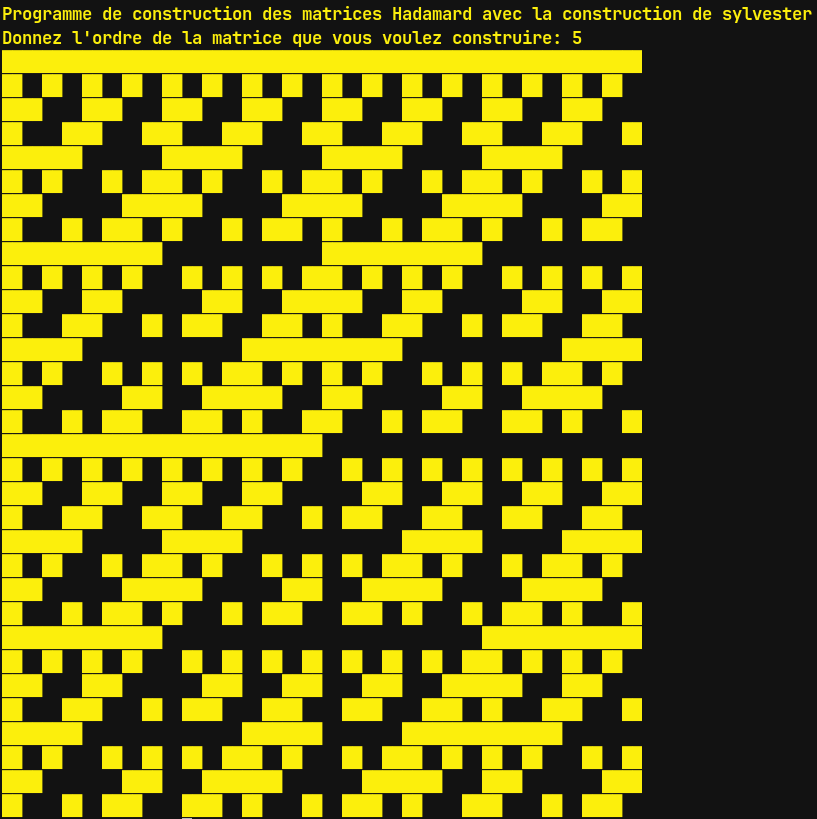
\includegraphics[width=\textwidth]{sylvester.png}
    \caption{Une matrice de Hadamard construite avec la construction de sylvestre}
  \end{center}
\end{figure}

\newpage
\subsubsection{Construction de Paley}

\paragraph{Définition}

La construction de Paley est une méthode de construction des matrices 
Hadamard en utilisant des corps finis qui a été décrit par le mathématicien
Raymond Paley en 1933.

\textbf{Note:} Un corps fini (aussi appellé corps de Galois) $K$ est un 
ensemble muni des opérations $(+, *)$ telles que:
\begin{itemize}
	\item $(K, +, *)$ est un anneau commutatif unitaire.
	\item $(K\setminus\{0_K\}, *)$ est un groupe.
	\item Le cardinal de $K$ est fini.
\end{itemize}

Soit $q$ une puissance d'un nombre premier impair et soit $F_q$ un corps 
fini de cardinal $q$ on définie le caractère quadratique $X(a)$ aussi 
appelé symbol de Legendre qui indique si l'élément $a$ est nul, un carré 
parfait non nul ou pas un carré parfait est définie formellement par:

\begin{equation*}
	X(a) = 
	\begin{cases}
		1 & \text{si a est un carré parfait module p et } 
		a \not\equiv 0 \pmod{p}\\
		-1 & \text{si a n'est pas un carré parfait modulo p}\\
		0 & \text{si } a \equiv 0 \pmod{p}
	\end{cases}
\end{equation*}

Exemple: Dans $F_5$, on a $X(4) = 1$ car  $3^2 \equiv 4 \pmod{5}$, 
$X(2) = -1$ car aucun élément au carré de $F_5$ n'est égal à 2.

On a:
\begin{itemize}
	\item $X(0) = 0$
	\item $X(1) = X(4) = 1$
	\item $X(2) = X(3) = -1$
\end{itemize}

\subparagraph{La matrice de Jacobsthal}

La matrice de Jacobsthal $Q$ dans $F_q$ est une matrice de taille $q*q$ 
dont les coefficients sont déterminés par le caractère quadratique de la 
différence entre les index des lignes et des colonnes c'est à dire:
$\text{ pour } a, b \in F_q \text{ alors } Q_{a,b} = X(a-b).$

D'aprés les valeurs obtenue à l'exemple précédent on obtient:
\begin{equation*}
	\begin{bmatrix}
		0 & 1 & -1 & -1 & 1\\
		1 & 0 & 1 & -1 & -1\\
		-1 & 1 & 0 & 1 & -1\\
		-1 & -1 & 1 & 0 & 1\\
		1 & -1 & -1 & 1 & 0
	\end{bmatrix}
\end{equation*}

\paragraph{Vers des matrices Hadamard}

On distingue deux cas selon le résultat de $q \pmod 4$:
\begin{itemize}
	\item $q \equiv 3 \pmod{4}:$
		\begin{equation*}
			\mathcal{H}_{q+1} = \mathcal{I}_{q+1} + 
			\begin{bmatrix}
				0 & j^T\\
				-j & \mathcal{Q}
			\end{bmatrix}
		\end{equation*}
		ou $\mathcal{I}$ est la matrice identité, $j$ le vecteur colonne de taille $q$
		avec uniquement des 1, $\mathcal{Q}$ est la matrice de Jacobsthal de taille 
		$q*q$.On obtient ainsi une matrice d'Hadamard de 
		taille $q+1$.
	\item $q \equiv 1 \pmod{4}:$\\
		On construit $\mathcal{H}_{2(q+1)}$ à partir de 
		$\begin{bmatrix}
			0 & j^T\\
			j & \mathcal{Q}
		\end{bmatrix}$.
		On remplace tous les 0 par la matrice
		$\begin{bmatrix}
			1 & -1\\
			-1 & -1
		\end{bmatrix}$,
		les 1 par 	
		$\begin{bmatrix}
			1 & 1\\
			1 & -1
		\end{bmatrix}$ 
		et les -1 par 
		$\begin{bmatrix}
			-1 & -1\\
			-1 & 1
		\end{bmatrix}$.On obtient ainsi une matrice d'Hadamard de taille 
		$2(q+1)$.
\end{itemize}

Poursuivons avec notre exemple, on a $5 \equiv 1 \pmod{4}$ donc nous somme
dans le cas 2:

\begin{equation*}
	\begin{bmatrix}
		0 & j^T\\
		j & Q
	\end{bmatrix}
	=
	\begin{bmatrix}
		0 & 1 & 1 & 1 & 1 & 1\\
		1 & 0 & 1 & -1 & -1 & 1\\
		1 & 1 & 0 & 1 & -1 & -1\\
		1 & -1 & 1 & 0 & 1 & -1\\
		1 & -1 & -1 & 1 & 0 & 1\\
		1 & 1 & -1 & -1 & 1 & 0
	\end{bmatrix}
\end{equation*}
en remplaçant les 0, 1 et -1 par les valeurs appropriées on obtient:

\setcounter{MaxMatrixCols}{20}

\begin{equation*}
	\mathcal{H}_{12}
	=
	\begin{bmatrix}
		1  & -1 & 1  & 1  & 1  & 1  & 1 & 1  & 1   &  1 & 1  & 1  \\
		-1 & -1 & 1  & -1 & 1  & -1 & 1 & -1 & 1   & -1 & 1  & -1 \\
		1  & 1  & 1  & -1 & 1  & 1  & -1 & -1 & -1 & -1 & 1  & 1  \\
		1  & -1 & -1 & -1 & 1  & -1 & -1 & 1  & -1 & 1  & 1  & -1 \\
		1  & 1  & 1  & 1  & 1  & -1 & 1  & 1  & -1 & -1 & -1 & -1 \\
		1  & -1 & 1  & -1 & -1 & -1 & 1  & -1 & -1 & 1  & -1 & 1  \\
		1  & 1  & -1 & -1 & 1  & 1  & 1  & -1 & 1  & 1  & -1 & -1 \\
		1  & -1 & -1 & 1  & 1  & -1 & -1 & -1 & 1  & -1 & -1 & 1  \\
		1  & 1  & -1 & -1 & -1 & -1 & 1  & 1  & 1  & -1 & 1  & 1  \\
		1  & -1 & -1 & 1  & -1 & 1  & 1  & -1 & -1 & -1 & 1  & -1 \\
		1  & 1  & 1  & 1  & -1 & -1 & -1 & -1 & 1  & 1  & 1  & -1 \\
		1  & -1 & 1  & -1 & -1 & 1  & -1 & 1  & 1  & -1 & -1 & -1
	\end{bmatrix}
\end{equation*}

On pouvez obtenir une matrice $\mathcal{H}_{12}$ avec $q = 11$ en utilisant le cas 1 
car $11 \equiv 3 \pmod{4}$.

\section{Codage}

\subsection{Démarches à suivre}

Le code de Hadamard est une technique de codage qui permet de transmettre
de l'information de manière robuste et résiliente aux erreurs.

Pour coder une information on commence par la coder en une séquence binaire,on avait 
mentionné que la taille du code Hadamard d'une séquence binaire 
de taille $k$ est $2^k$ donc aprés avoir construit le vecteur binaire à 
partir de la séquence binaire de l'information on construit la matrice de
Hadamard de taille $2^k$ et le code sera généré en utilisant les lignes de la matrice en 
associant d'une façon bijective chaque mot de code à une ligne de la matrice.

Supposons par exemple que notre alphabet de départ est $\mathcal{A} = {a, b, c, d, e, d, g
, h}$ qui peut être codé en binaire sur 3 bits, pour coder chaque lettre avec un code 
Hadamard il faut construire une matrice d'Hadamard de taille $2^3=8$ et il faut établir une
bijection entre chaque lettre et chaque ligne dans la matrice résultante.

\begin{center}
\begin{tabular}{c|c|c}
	\hline 
	lettre & codage binaire & codage Hadamard \\
	\hline
	a & 000 & 1 1 1 1 1 1 1 1 \\
	\hline
	b & 001 & 1 -1 1 -1 1 -1 1 -1 \\
	\hline
	c & 010 & 1 1 -1 -1 1 1 -1 -1 \\
	\hline 
	d & 011 & 1 -1 -1 1 1 -1 -1 1 \\
	\hline 
	e & 100 & 1 1 1 1 -1 -1 -1 -1 \\
	\hline 
	f & 101 & 1 -1 1 -1 -1 1 -1 1 \\
	\hline 
	g & 110 & 1 1 -1 -1 -1 -1 1 1 \\
	\hline 
	h & 111 & 1 -1 -1 1 -1 1 1 -1 \\
	\hline
\end{tabular}
\end{center}

Si on veut coder par exemple le mot "abab", on procéde en concaténant le codage Hadamard de
chaque lettre et on obtient: 
1 1 1 1 1 1 1 1 1 -1 1 -1 1 -1 1 -1 1 1 1 1 1 1 1 1 1 -1 1 -1 1 -1 1 -1
ce qui explique pourquoi le taux de transfert de ce code est extrêmement faible.

\subsection{Algorithme}
\vspace{1em}

\begin{algorithm}
\caption{Codage Hadamard}
	\textbf{Entrées:} un alphabet $A$ à coder\\
    \textbf{Sortie:} le code Hadamard de 
	l'alphabet
	\begin{algorithmic}
		\State $k \gets $ taille($A$) 
		\State $\mathcal{H}_{2^k} $= matrice\_hadamard($k$)
		\For{i de 1 à k}
			\State $code[i] \gets \mathcal{H}_{i}$
		\EndFor
		\State renvoyer code
	\end{algorithmic}
\end{algorithm}

\section{Decodage}

L'efficacité du décodage des codes Hadamard réside dans leur capacité à 
détecter et à corriger les erreurs tout en maintenant une complexité 
algorithmique raisonnable. L'utilisation de propriétés mathématiques 
avancées, combinée à la structure particulière des matrices de Hadamard, 
permet d'obtenir des performances de correction d'erreur élevées tout en 
minimisant la complexité des algorithmes de décodage.

Dans cette perspective, l'introduction de codes Hadamard dans les systèmes 
de communication offre une robustesse significative contre les erreurs de 
transmission, contribuant ainsi à l'amélioration de la fiabilité des 
échanges d'informations dans des environnements où le bruit et les 
perturbations sont inévitables.

\subsection{Démarches à suivre}
Pour décoder un mot de code codé avec le code Hadamard décrit précèdemment on se base sur
le spectre des matrices d'Hadamard et plus précisément sur la plus grande valeur dans les 
valeurs spéctrales qu'on obtient en multipliant le mot de code reçu $c$ avec une matrice 
d'Hadamard d'ordre la taille de ce mot de code, et pour décoder un message complet il faut
répéter la même procédure pour chaque mot de code dans le code reçu.

Supposons qu'on a reçu le code suivant codé avec le codage précèdent:
1 1 1 1 1 1 1 1 1 -1 -1 -1 1 -1 1 -1 

chaque mot de code est de taille 8 donc le premier mot de code est: 1 1 1 1 1 1 1 1 et le 
deuxieme est: 1 -1 -1 -1 1 -1 1 -1, en multipliant le premier mot de code avec 
$\mathcal{H}_8$ on obtient:
\begin{equation*}
	d = [1, 1, 1, 1, 1, 1, 1, 1] \times \mathcal{H}_8 = [8, 0, 0, 0, 0, 0, 0, 0]
\end{equation*}
La plus grande valeur dans le vecteur d est 8 qui se trouve à la premiére position ce qui 
correspond dans notre table de bijection à la lettre a; pour le deuxième mot de code on 
obtient:
\begin{equation*}
	d = [1, -1, -1, -1, 1, -1, 1, -1] \times \mathcal{H}_8 = [-2, 6, 2, 2, -2, -2, 2, 2]
\end{equation*}
La plus grande valeur dans le vecteur d est 6 qui se trouve à la deuxième position ce qui 
correpond à la lettre b dans la table de bijection donc le mot de code: 
1 -1 -1 -1 1 -1 1 -1 code la lettre b, on remarque que toutes les autres valeurs ne sont 
pas nuls ce qui signifie que le mot de code reçu est modifié et c'est comme ça que le code
permet de détécter les erreurs dans les messages reçus, et dans notre cas de corriger 
une seule erreur car le mot b est sencé être codé sur: 1 -1 1 -1 1 -1 1 -1, en utilisant la
formule fourni dans la section d'introduction 1.2 avec $k=3$ notre code sera capable de 
corriger seulement une erreur et capable de détecter jusqu'à 4 erreurs simples.
\newpage
\subsection{Algorithme}
\vspace{1em}
\begin{algorithm}[h]
\caption{Décodage d'un mot de code Hadamard}
	\textbf{Entrées:} un mot de code $c$ à décoder\\
    \textbf{Sortie:} le message décodé 
	\begin{algorithmic}
		\State $k \gets $ taille($c$)
		\State $d \gets $ tableau de taille $k$
		\State $\mathcal{H}_{k} $= matrice\_hadamard($log(k)$)
		\For{i de 1 à k}
			\State $d[i] \gets \sum_{j=1}^{k} c[i] * \mathcal{H}[i][j]$
		\EndFor
		\State $pos \gets $ position de la plus grande valeur dans d
		\State $m \gets $ lettre correspondante à la position $pos$ dans la table de 
		bijection construite dans le codage 
		\State renvoyer $m$
	\end{algorithmic}
\end{algorithm}
\vspace{1em}

\subsection{Propriété Localement déchiffrable}
La propriété de localement déchiffrable est une propriété intéressante pour les codes 
correcteurs d'erreurs, tels que le code de Hadamard. Un code est dit localement 
déchiffrable s'il est possible de décoder chaque position individuellement sans avoir 
besoin de déchiffrer l'ensemble du message.

Pour le code de Hadamard, cette propriété signifie que si une petite partie du message est
corrompue (quelques bits ont été modifiés), il est possible de corriger ces erreurs en ne 
consultant que la portion du message affectée, sans avoir besoin de regarder le message 
entier.
\newpage

\begin{figure}[h]
  \centering
  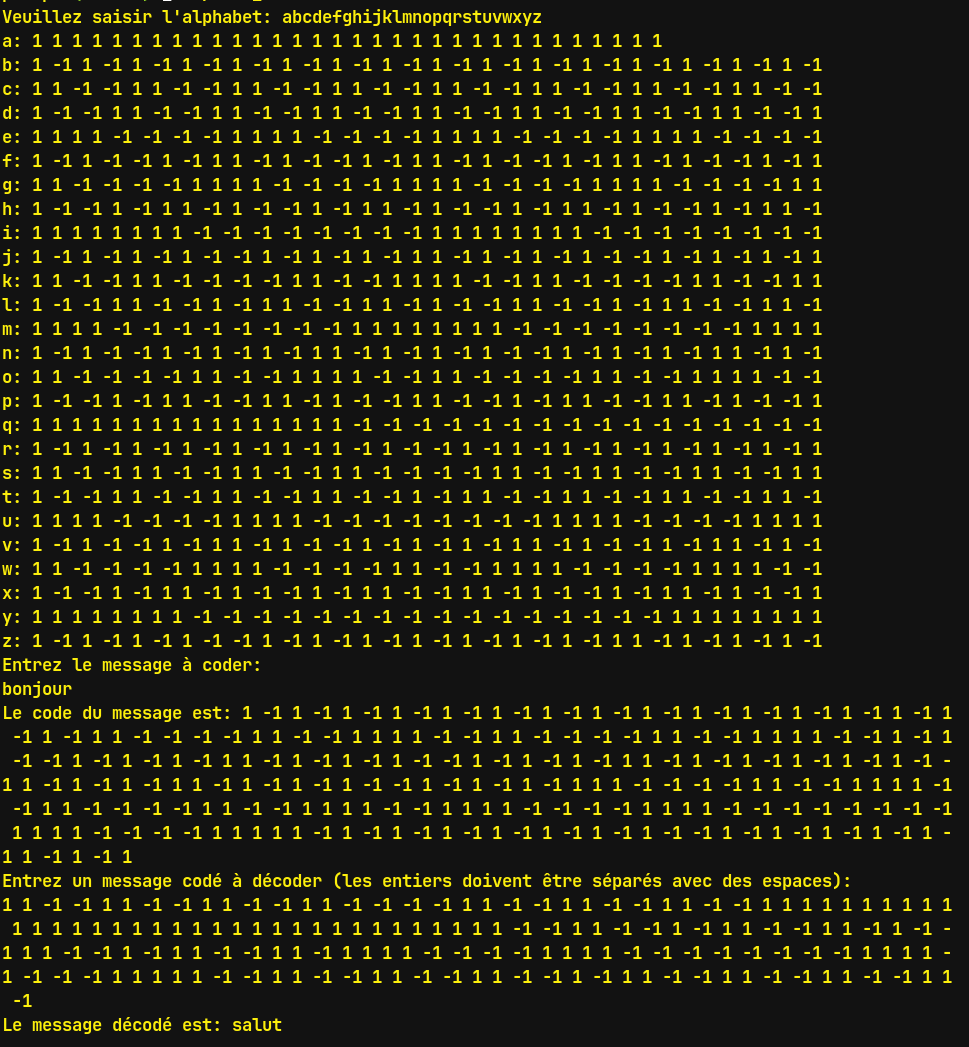
\includegraphics[width=1\textwidth]{code_decode.png}
  \caption{example d'éxécution du programme de codage et décodage}
  \label{codage décodage}
\end{figure}

\newpage
\section*{annexe}
\begin{itemize}
	\item \href{https://www.matec-conferences.org/articles/matecconf/pdf/2017/39/matecconf_cscc2017_05007.pdf}{Application of Enhanced Hadamard Error Correcting Code in 
		Video-Watermarking and his comparison to Reed-SolomonCode.}
	\item \href{https://math.univ-lille1.fr/~calgaro/TER_2018/wa_files/maire.pdf}
		{Matrices de Hadamard et Applications.}
	\item \href{http://jacquescellier.fr/maths/matrices_hadamard.pdf}
		{Autour des Matrices de Hadamard}
	\item \href{https://books.google.fr/books?hl=en&lr=&id=XaV7CwAAQBAJ&oi=fnd&pg=PA1&dq=le+code+de+hadamard&ots=lTY7NYeAOB&sig=PHyTnem5GyCK9jHSHf1WRQxGV_M&redir_esc=y#v=onepage&q=le\%20code\%20de\%20hadamard&f=false}
		{Hadamard Matrices and Their Applications}
	\item \href{https://fr.wikipedia.org/wiki/Code_de_Hadamard}{Code de Hadamard}
\end{itemize}
\end{document}
